%
% Szakdolgozatminta az Eszterházy Károly Katolikus Egyetem
% matematika illetve informatika szakos hallgatóinak.
%

\documentclass[
% opciók nélkül: egyoldalas nyomtatás, elektronikus verzió
% twoside,     % kétoldalas nyomtatás
% tocnopagenum,% oldalszámozás a tartalomjegyzék után kezdődik
]{thesis-ekf}
\usepackage[T1]{fontenc}
\PassOptionsToPackage{defaults=hu-min}{magyar.ldf}
\usepackage[magyar]{babel}
\usepackage{mathtools,amssymb,amsthm,pdfpages, listingsutf8, xcolor, caption}
\footnotestyle{rule=fourth}

\newtheorem{tetel}{Tétel}[chapter]
\theoremstyle{definition}
\newtheorem{definicio}[tetel]{Definíció}
\theoremstyle{remark}
\newtheorem{megjegyzes}[tetel]{Megjegyzés}

\renewcommand{\lstlistingname}{kód}
\lstdefinestyle{csharp}{
	inputencoding=utf8/latin2,
	language=[Sharp]C,
	basicstyle=\footnotesize,
	numbers=left,
	xleftmargin=1cm,
	xrightmargin=1cm,
	breaklines,
	postbreak=\hbox{$\color{red}\hookrightarrow\ $},
	backgroundcolor=\color{gray!30},
	frame=tblr,
	framesep=3pt,
	commentstyle=\itshape\color{teal},
	keywordstyle=\bfseries\color{blue},
}

\definecolor{maroon}{rgb}{0.5,0,0}
\definecolor{darkgreen}{rgb}{0,0.5,0}


\lstdefinestyle{xml}{
	inputencoding=utf8/latin2,
	language=XML,
	basicstyle=\footnotesize,
	numbers=left,
	xleftmargin=1cm,
	xrightmargin=1cm,
	breaklines=true,
	postbreak=\hbox{$\color{red}\hookrightarrow\ $},
	backgroundcolor=\color{gray!30},
	frame=tblr,
	framesep=3pt,
	commentstyle=\color{teal},
	morecomment=[s]{<!--}{-->},
	keywordstyle=\bfseries\color{blue},
}
\begin{document}
\institute{Matematikai és Informatikai Intézet}
\title{Árgép robot fejlesztése}
\author{Kis Sándor\\Programtervező Informatikus BSc}
\supervisor{Nagy Péter\\Külső konzulens}
\city{Eger}
\date{2024}
\maketitle
\tableofcontents

\chapter*{Bevezetés}
\addcontentsline{toc}{chapter}{Bevezetés}
A mindennapi munkám során számos ismétlődő feladatokat kell elvégeznem a számítógépen. Ezek a tevékenységek általában adatbevitellel és különböző, ugyanarra a sablonra épülő riportok elkészítésével kapcsolatosak. Az ilyen típusú feladatok igen időigényesek, Én naponta akár több munkaórát is ezekre fordítok. Az így eltöltött időt sokkal értékesebben is fel tudnám használni, ezáltal sokkal hatékonyabban tudnám elvégezni a munkámat.

Gondolom, nagyon sokan vannak hasonló helyzetben, olyanok akik egyhangú, monoton, ismétlődő munkát végeznek számítógépen. Ezeknek az ismétlődő munkafolyamatoknak az automatizálásával rendkívüli hatékonyságot lehet elérni úgy, hogy rengeteg munkaórát lehet megtakarítani, és még a hibalehetőségeket is a minimálisra lehet csökkenteni. Az automatizálásra számos megoldás létezik. A UiPath kiemelkedik ezen a területen és a robotfolyamat-automatizáció (RPA) terén kiváló megoldásokat kínál.

A UIPath által létrehozott technológia kulcsfontosságú szerepet játszik a munkafolyamatok automatizálásában. Azokon a területeken, ahol az ismétlődő feladatok és a rutinszerű folyamatok gyakran előfordulnak, az RPA segítségével rendkívül hatékonyan lehet robotokat alkalmazni. Például az adatbevitel, az adatellenőrzés és különböző adminisztratív folyamatok és feladatok automatizálásával az UiPath robot gyors, hatékony és precíz műveleteket végez szinte hibatlanul.

Egy másik lényeges dolog az RPA alkalmazásában az, hogy a UiPath rendszer egyszerüen lehetővé teszi az integrációt más vállalati rendszerekkel. Ez azt jelenti, hogy a meglévő informatikai infrastruktúrát könnyen kombinálhatjuk a automatizálással, anélkül, hogy nagyobb es kötséges átalakításokra lenne szükség. Ez lehetővé teszi a vállalatok számára, hogy fokozatosan vezessék be az automatizációt, kezdve a legkritikusabb területekkel, majd később kiterjeszthetik azt az egész vállalati környezetre.

Az automatizáció tehát nemcsak, hogy meggyorsítja a munkafolyamatokat, de elősegíti a vállalati hatékonyságot és az emberi erőforrások felszabadítását,  ezáltal javíta a vállalatok versenyképességét. Azok a vállalatok, amelyek hatékonyan alkalmazzák az automatizációt, hatalmas előnyt szerezhetnek a versenytársaikkal szemben a folyamatosan változo piaci környezetben.


\section*{Célkitűzés}
A szakdolgozatom elkészítése során a UiPath technológiát felhasználva létrehoztam egy Árgép robotot, ami segít összeállítani egy asztali PC-t a lehető legolcsóbb áron. Az Árgép robot egy adatbázisból dolgozik, amelyben tárolva vannak az alkatrészek és a webshopok információi. 

A felhasználók egyszerűen felsorolják a kívánt alkatrészeket egy Excel fájlban, amelyet egy asztali alkalmazás segítségével feltöltenek az adatbázisba, majd elindítják a robotot. A robot az adatbázisból kiolvassa az információkat, majd leellenőrzi a webshopokat az alkatrészek aktuális áraiért. Végül a robot riportot készít, amelyben összehasonlítást nyújt arról, hogy melyik webshopban találhatók a legolcsóbb alkatrészek, majd ezt a riportot emailben elküldi a felhasználónak.


\chapter{Választott technológiák bemutatása}
\section{.NET Keretrendszer \cite{.NET}}
.NET-keretrendszer egy olyan technológia, amely támogatja a Windows-alkalmazások és webszolgáltatások készítését és futtatását. Előzőleg a .NET nemcsak fejlesztői környezetet jelentett, hanem magában foglalta különböző szoftvereket, fejlesztőeszközöket és hardvereszközöket is, azonban ma már a .NET kifejezés kizárólag magára a keretrendszerre vonatkozik.

.NET-keretrendszer a közös nyelvi futtatókörnyezetből (CLR) és a .NET- keretrendszer osztálytárból áll. A közös nyelvi futtatókörnyezet a .NET- keretrendszer alapja. Végrehajtáskor kezeli a kódot és olyan alapvető szolgáltatásokat nyújt, mint a memóriakezelés, a szálkezelés és a visszalépés, miközben szigorú típusbiztonságot és a kód pontosságának egyéb olyan formáit is kikényszeríti, amelyek elősegítik a biztonságot és a robusztusságot.

Az osztálytár olyan újrafelhasználható típusok átfogó, objektumorientált gyűjteménye, amellyel a hagyományos parancssori vagy grafikus felhasználói felületi (GUI) alkalmazásoktól kezdve az ASP.NET által biztosított legújabb innovációkon alapuló alkalmazásokig, például Web Forms és XML-webszolgáltatásokig terjedő alkalmazásokat fejleszthetők.

A Microsoft a .NET platform kiadásakor bevezetett egy új programozási nyelvet, a C\#-ot. Ez a programozási nyelv egy letisztult szintaxissal rendelkező nyelv, melynek alapjait más, sikeres nyelvek vetették meg. A Microsoft egyszerűen áttekintette a legelterjedtebb programozási nyelveket, sorra vette azok minden jó tulajdonságát és hibáját. A C\#-ban igyekeztek a jó tulajdonságokat maximalizálni, a rosszakat minimalizálni. Fontos megjegyezni, hogy a C\# egy tisztán OOP (objektumorientált programozási) nyelv, ezzel átlépve az egyik legnépszerűbb programozási nyelv, a C++ korlátait.
\section{Entity Framework \cite{Entity}}
Az Entity Framework egy objektum-relációs leképző (ORM) keretrendszer, amely lehetővé teszi a fejlesztők számára, hogy objektumorientált módon dolgozzanak relációs adatbázisokkal. Ez azt jelenti, hogy a fejlesztők az adatbázis-táblákat objektumokként kezelhetik, és nem kell SQL-utasításokat írniuk az adatok lekérdezéséhez és módosításához. Az Entity Framework kulcsfontosságú előnyei közé tartozik a megnövelt termelékenység, a kód egyszerűsítése és a kiváló hibaelhárítási képességek. 

A .NET-alapú alkalmazások fejlesztéskor, amikor adatbázis-hozzáférésre van szüksége, az Entity Framework kiváló választás.
\section{Windows Presentation Foundation}
A Windows Presentation Foundation (WPF) egy grafikus felhasználói interfész (GUI) keretrendszer, amelyet a Microsoft fejlesztett ki Windows alkalmazások készítéséhez. A WPF segitségével esztétikus, interaktív és gazdag felhasználói élményt kínáló alkalmazások fejlesztese lehetseges.
\subsection*{WPF néhány jellemzője:}
\begin{itemize}
	
	\item \textbf{Deklaratív XAML (eXtensible Application Markup Language):} 
	A WPF az XML-alapú XAML-t használja az alkalmazások felhasználói interfészének deklaratív leírásához. Ez lehetővé teszi a tervezők és fejlesztők számára, hogy könnyen elkészítsék és szerkesszék a felhasználói felületet.
	\item \textbf{Adatkötés (Data Binding)}: Lehetővé teszi az adatok dinamikus kapcsolatát a felhasználói interfésszel. Az adatkötés segítségével az adatok automatikusan frissülnek, amikor azok megváltoznak, és így az alkalmazások dinamikusabbak és interaktívabbak lehetnek.
	\item \textbf{Stílusok és Sablonok (Styles and Templates):} A WPF lehetővé teszi a felhasználói interfész elemeinek stílusainak és sablonjainak egyszerű definiálását és alkalmazását. Ez segíti a dizájn egységesítését és az alkalmazások testreszabhatóságát.
	\item \textbf{Vektorgrafika és Animációk:} A WPF támogatja a vektorgrafikát, amely lehetővé teszi a skálázható és magas felbontású grafikai elemek használatát. Emellett a keretrendszer könnyen kezeli az animációkat is.
\end{itemize}
\section{MVVM (Model-View-ViewModel)}
Az MVVM egy olyan tervezési minta, amelyenek célja az alkalmazások strukturáltabbá tétele és könnyebb karbantarthatósága. A nevét a három fő komponensének nevéből kapta:
\begin{itemize}
	
	\item \textbf{Model:} A Model reprezentálja az alkalmazás üzleti logikáját és adatelérési rétegét. Ez a rész felelős az adatok kezeléséért és az üzleti szabályok végrehajtásáért.

	\item \textbf{View:} A View felelős a felhasználói felület megjelenítéséért. Ez a rész megjeleníti az adatokat és érzékeli a felhasználói interakciókat.

	\item \textbf{ViewModel:} A ViewModel egy köztes réteg a Model és a View között. Feladata a felhasználói felület és az üzleti logika közötti kapcsolat fenntartása. A ViewModel feldolgozza a felhasználói interakciókat a View-tól, valamint frissíti a View-t az adatokból, amelyeket a Modelből kap. A ViewModel segítségével az alkalmazás jól elkülöníthető módon oszlik meg, ami könnyebb tesztelést és karbantarthatóságot eredményez.
\end{itemize}
Az MVVM használatával az alkalmazás könnyebben bővíthető és karbantartható, és lehetőséget ad az egységtesztekre is. A WPF keretrendszer kifejezetten támogatja az MVVM tervezési mintát, és könnyen kezelhető adatkötést kínál a View és a ViewModel között.
	\begin{figure}[!ht]
		\centering
		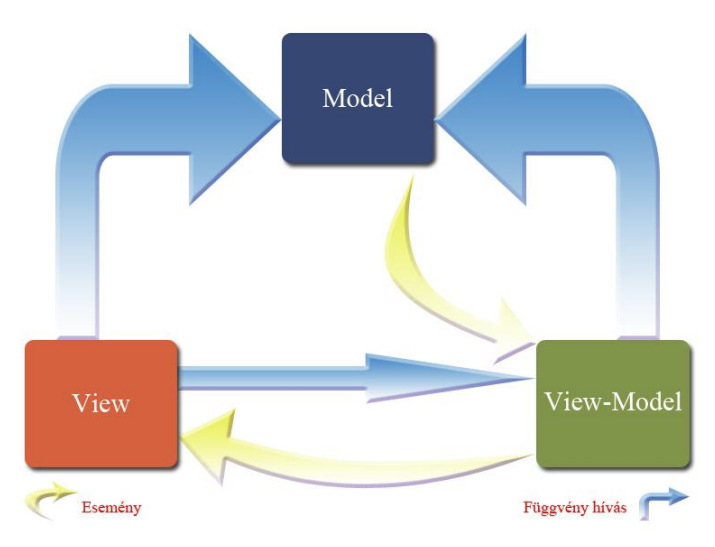
\includegraphics[width=12cm]{mvvm}
		\caption{Az MVVM modell \cite{Progtech}}
		\label{picture-mvvm}
	\end{figure}

\section{Microsoft SQL Server}
A Microsoft SQL Server a Microsoft által kifeljesztett relációs adatbázis-kezelő rendszer, mely az SQL (Structured Query Language) nyelvet használja az adatok tárolására, lekérdezésére és kezelésére. 

A SQL Server eredetileg kifejezetten a Windows operációs rendszerre lett tervezve, de az újabb verziók már támogatják más operációs rendszereken való futtatást is, például Linuxon és Docker konténerekben, ezáltal rugalmasságot biztosítanak a különböző környezetekben történő telepítéshez és üzemeltetéshez.

Az SQL Server Management Studio (SSMS) egy grafikus felhasználói felület (GUI), mely segíti a felhasználókat a Microsoft SQL Server adatbázis-kezelő rendszerével kapcsolatos feladatok egyszerű és hatékony végrehajtásában. Az SSMS lehetővé teszi az adatbázisok tervezését, létrehozását, karbantartását és felügyeletét, valamint a lekérdezések írását és futtatását.
\section{UiPath}
UiPath története 2005-re nyúlik vissza, ekkor alapította meg a DeskOver vállalatot Daniel Dines és Marius Tirca egy bukaresti lakásban. Kezdetben szoftverautomatizációs eszközöket és fejlesztői készleteket hoztak létre olyan neves cégek számára, mint az IBM, a Google és a Microsoft, akik ezeket beépítették saját termékeikbe. 

Az igazi áttörés 2012-ben jött el, ekkor találó módon egy ügyfél volt az, aki rámutatott a kezdetleges RPA (robotfolyamat-automatizálás) piacon rejlő lehetőségekre a cég számára.

2013-ban a cég piacra dobta az első UiPath Desktop Automation termékcsaládot, amely eszközöket biztosított a vállalatok számára az adminisztratív, ismétlődő feladatok automatizálásához. A vállalat életében a következő mérföldkő az 2015-ös év volt. Ekkor mutatták be az új vállalati platformot, és ekkor vette fel a cég a UiPath nevet is.

A UiPath hamarosan vezető szereplővé vált az RPA piacon, és az általuk kifejlesztett eszközök és szolgáltatások kiválóan segítették a vállalatokat az üzleti folyamatok hatékonyabbá és termelékenyebbé tételében. A UiPath termékei között szerepel a UiPath Studio, ami a fejlesztőknek segít az automatizációs feladatok létrehozásában és kezelésében, valamint a UiPath Orchestrator, egy eszköz a robotok menedzselésére és ellenőrzésére.

A UiPath jelenlegi célkitűzése a Fully Automated Enterprise - a teljesen automatizált vállalat - koncepciójának megvalósítása. Ennek révén a vállalatok teljes mértékben kiaknázhatják bennük rejlő lehetőségeket az automatizáció segítségével, felszabadítva az emberi munkaerőt a kreatívabb feladatok elvégzésére.

\subsection{ UiPath Studio}
A UiPath Studio a UiPath vállalati RPA platformjának központi eleme, egy vizuális fejlesztői környezet, amely lehetővé teszi automatizált munkafolyamatok egyszerű és gyors létrehozását. Ez azt jelenti, hogy felhasználóknak nem kell kódolási ismeretekkel rendelkezniük a használatához. Akár üzleti felhasználók, akár fejlesztők számára hasznos eszköz, különböző automatizálási igények megoldására.
\subsection*{Studio főbb jellemzői:}
	\begin{itemize}
		\item \textbf{Vizuális fejlesztés:} Egyszerűen összeállíthatók automatizált munkafolyamatok különféle tevékenységekből, mint például az alkalmazás indítása, adatok bevitele, adatgyűjtés, döntéshozatal stb. a drag-and-drop funkcióknak köszönhetően.
		
		\item \textbf{Felvett tevékenységek:} Rögzíthetjük a manuális műveleteket, majd a Stúdióban lejátszhatjuk és finomhangolhatjuk azokat automatizációs feladatokká.
				
		\item \textbf{Kiterjedt tevékenységpaletta:} Számos előre definiált tevékenység áll rendelkezésre különböző automatizálási célokra, például webes, asztali és Citrix alkalmazásokhoz, adatmanipulációhoz, hibakezeléshez stb.
		
		
		\item \textbf{Változó szintű komplexitás:} Egyszerű automatizációk készítése kezdő felhasználók számára, míg a tapasztaltabbak összetettebb munkafolyamatokat is létrehozhatnak.
		
		\item \textbf{Hibakezelés:} Beállíthatók hibakezelési lépések, hogy az automatizáció megfelelően reagáljon váratlan események esetén.
		
		\item \textbf{Logok és audit naplók:} Részletes naplókat készíthetünk a munkafolyamatok végrehajtásáról, ami segít a hibakeresésben és a monitoringban.
		
		\item \textbf{Integráció más eszközökkel:} Könnyen integrálható más RPA komponensekkel, AI funkciókkal, harmadik fél eszközökkel és API-kkal.
		
	\end{itemize}
\subsection*{Studio változatai:}
	\begin{itemize}
		\item \textbf{UiPath StudioX:} A Studio egyszerűsített változata, kezdőknek ajánlott.
		\item \textbf{UiPath Studio:} Teljes körű fejlesztői környezet, komplexebb automatizáláshoz.
		\item \textbf{UiPath Studio Web:} Webalapú fejlesztői környezet, online alkalmazások automatizálására.
	\end{itemize}

	
\subsection{ UiPath Orchestrator}
Az UiPath Orchestrator a UiPath vállalati RPA platformjának egy másik kulcsfontosságú eleme. Ez egy központi vezérlőpult, amely lehetővé teszi az RPA-folyamatok ütemezését, figyelését, kezelését és skálázását. Gyakorlatilag az Orchestrator felel az automatizált munkafolyamatok életciklusának teljes körű felügyeleteért.

\subsection*{Orchestrator főbb jellemzői:}
\begin{itemize}
		\item \textbf{Központi irányítás:} Lehetővé teszi az összes RPA robot és munkafolyamat felügyeletét egyetlen helyről.
		\item \textbf{Ütemezés és indítás:} Automatizált munkafolyamatok ütemezése meghatározott időpontokra, eseményekre vagy igényekre reagálva.
		\item \textbf{Monitoring:} Valós időbeli betekintést nyújt futó és befejezett munkafolyamatról. Láthatjuk az aktuális állapotot, a végrehajtási időt, a feldolgozott adatok mennyiségét, valamint bármilyen hibaüzenetet vagy figyelmeztetést.
		\item \textbf{Teljesítménymutatók:} Az Orchestrator számos előre definiált teljesítménymutatót (KPI) kínál, amelyek segítségével követni tudjuk a  munkafolyamatainak hatékonyságát és sikerességét.
		\item \textbf{Riportálás:} Beépített jelentéskészítő eszközöket tartalmaz, amelyekkel könnyen létrehozhatók és exportálhatók jelentések a munkafolyamatok teljesítményéről, hibákról és trendekről.
		\item \textbf{Biztonsági hozzáférés-vezérlés:} Lehetővé teszi hozzáférési szintek beállítását a felhasználók számára a biztonságos és ellenőrzött működés érdekében.
\end{itemize}
\subsection*{Orchestrator előnyei:}
\begin{itemize}
		\item \textbf{Megnövelt hatékonyság:} Automatizált folyamatok központosított kezelésével csökkenti a manuális felügyeleti terheket és növeli a hatékonyságot.
		\item \textbf{Jobb láthatóság:} valós dőbeli betekintést nyújt munkafolyamatok teljesítményébe, lehetővé téve a hibák gyors azonosítását és megoldását.
		\item \textbf{Skálázhatóság:} Könnyedén skálázható a platform a növekvő automatizálási igényeknek megfelelően.
		\item \textbf{Biztonság:}  Biztonságos környezetet biztosít az RPA-folyamatok futtatásához, megfelelve a vállalatok biztonsági előírásaiknak.
\end{itemize}
\subsection{ UiPath Robot}
Az UiPath Robot egy szoftverrobot, mely a számítógépen elvégzi az automatizált, ismétlődő manuális feladatokat.  A robotot a UiPath Studio grafikus felületén fejleszthetjük ki, ahol a munkafolyamatokat programozhatjuk a robot számára. Az UiPath Robotnak két fő típusa van. A Felügyelt (attended) robot emberi beavatkozást igényel a munkafolyamatok futtatásához. A felhasználónak manuálisan kell elindítania a robotot, és meg kell adnia a szükséges bemeneteket. Felügyelet nélküli (unattended) robot önállóan futtatja a munkafolyamatokat, emberi beavatkozás nélkül. A robotot előre be kell konfigurálni a szükséges bemenetekkel és kimenetekkel.

\subsection*{A UiPath Robot főbb jellemzői:}
\begin{itemize}
\item\textbf{ Megbízható:} A UiPath Robot robusztus és megbízható, így a munkafolyamatok zökkenőmentesen futnak, minimális felügyelet mellett.
\item\textbf{Rugalmas:} A UiPath Robot széles skálájú feladatok automatizálására használható, beleértve az adatbevitelt, az adatkivonást, a webes kaparást, az e-mailek kezelését és a PDF-fájlok feldolgozását.
\item \textbf{Könnyen használható:} A UiPath Robot intuitív grafikus felülettel rendelkezik, így a kódolási ismeretek nélküli felhasználók is könnyen használhatják.
\item \textbf{Skálázható:} A UiPath Robot alkalmas nagyobb volumenű munkafolyamatok kezelésére is, így a vállalatok könnyen skálázhatják az automatizációs projektjeiket.
\item \textbf{Integrálható:} A UiPath Robot könnyen integrálható más üzleti alkalmazásokkal és rendszerekkel, lehetővé téve a szervezetek számára az egységes munkafolyamatok kialakítását.
\end{itemize}
\subsection{A UiPath fejlesztés alapjai:}
Mint már az előző fejezetben említettem, a fejlesztés a UiPath Studio grafikus felületén történik. Itt több száz előre elkészített activity található. Ezek az activity-k teszik lehetővé a különböző feladatok automatizálását. Ezek a feladatok lehetnek például adatbázis-műveletek, fájlok kezelése vagy webes feladatok, amelyeket automatizálni szeretnénk. Érdemes megjegyezni, hogy a beépített activity-ken kívül a Studio csomagkezelőjével külső fejlesztők által írt activity-ket is telepíthetünk, vagy akár saját magunk is írhatunk activity-ket. Ehhez a Microsoft Visual Studio fejlesztői környezete szükséges.  
\subsection*{Workflow-k UiPath-ban: \cite{Workflow}}
Az activity-ket drag and drop módszerrel egyszerűen munkafolyamatokba (workflow) szervezhetjük. Attól függően, hogy milyen feladatokat szeretnénk automatizálni, a UiPath a következő munkafolyamatokat kínálja:
\begin{itemize}
	\item\textbf{Sequence:} Egyszerű, lineáris workflow, amely felülről lefelé haladva, egymás után hajtja végre az activity-ket. Előnye, hogy egyszerű összeállítani, jól átlátható és könnyen olvasható. Legtöbbször elegendő is a kívánt feladat automatizálására.
	\item \textbf{Flowchart:} Vizuális workflow, akkor érdemes használni, amikor az automatizálási folyamat több elágazással, döntési csomóponttal rendelkezik. Ez a legjobb választás a nem lineáris folyamatok automatizálására. 
	\item \textbf{State Machine:}Ez egy összetettebb workflow, akkor érdemes használni, amikor a folyamat különböző állapotokat, úgynevezett state-eket vehet fel. A tranzakciók irányítják az állapotok változását, vagyis azt, hogy egyik state-ből mikor léphetünk tovább egy másikba. Minden tranzakció feltételhez kötött, és ha a feltétel teljesül, akkor aktiválódik a tranzakció, és a State Machine állapotot vált.
	\item \textbf{Global Exception Handler:}Ez egy speciális workflow, amely nem kezelt kivételek esetén automatikusan lefut. Használata segít az automatizálás megbízhatóságának növelésében.
\end{itemize}	
\subsection*{Activity-k UiPath-ban: \cite{Activity}}
Az activity-k a UiPath automatizálás alapvető építőkövei, amelyek reprezentálják azokat a műveleteket, amelyeket az automatizálás során végre szeretnénk hajtani. Minden egyes activity egy speciális funkciót hajt végre. Ilyen funkció lehet például egy e-mail küldése, egy űrlap adatokkal való kitöltése vagy egy adatbázis lekérdezés. Az activity-k paraméterekkel könnyen testreszabhatók, így az adott igényekhez alakíthatók.

	\begin{figure}[!ht]
	\centering
	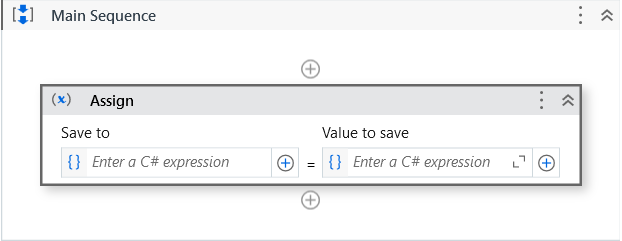
\includegraphics[height=5cm]{activity}
	\caption{Assign activity Sequence workflow-ban}
	\label{picture-activity}
\end{figure}

\chapter{Megoldás}
A projektem három fő részből áll. Az első rész egy REST API szerver, amely az ASP.NET Core keretrendszerre épül. A második rész egy desktop alkalmazás, amely elküldi az adatbázisba elmentendő adatokat a REST API-n keresztül a szervernek. Ezt az alkalmazást ExcelDataLoader-nek neveztem el, és a Windows Presentation Foundation keretrendszer segítségével készítettem el. A projekt harmadik része maga a UiPath Árgép robot, amely az automatizálási feladatokat látja el.
\section{REST API Szerver}
Ez a komponens biztosítja a kommunikációs felületet a kliensalkalmazás és az adatbázis között, lehetővé téve az adatbázis műveletek végrehajtását HTTP kéréseken keresztül.
\subsection{Adatbázis}
Az alkalmazásban nincs szükség sok adat tárolására, csupán a webáruházak nevét, webcímét, valamint a megvásárolni kívánt számítógép alkatrészekhez tartozó alapvető információkat kell eltárolni, illetve kiolvasni.Emellett a robot keresési eredményeit is el kell menteni az adatbázisba, majd a keresési eredmények közül a legolcsóbb alkatrészek adatait is ki kell nyerni.
	\begin{figure}[!ht]
		\centering
		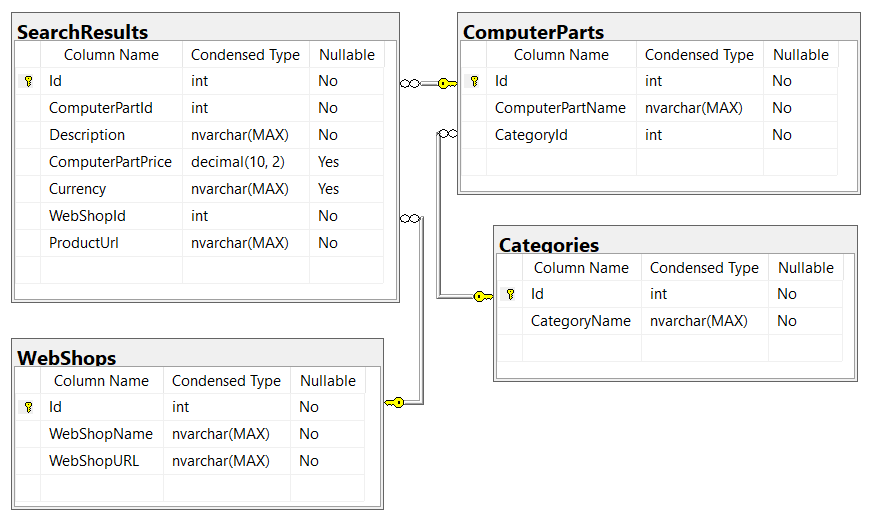
\includegraphics[width=15cm, height=7.5cm]{entity_diagram}
		\caption{SSMS adatbázis diagram}
		\label{picture-adatbazis}
	\end{figure}
Az adatbázis felépítése a az \ref{picture-adatbazis} ábrán látható. 

Az adatbázisban összesen négy tábla található: a ComputerParts, WebShops, és Categories táblákba az adatokat az Excel Data Loader asztali alkalmazás segítségével egyszerűen feltölthetjük egy Excel-fájlból.
A negyedik, egyben fő táblánk a SearchResults tábla, amelybe a robot az összes alkatrészről talált keresési eredményt elmenti majd el. Ebben a táblában két idegen kulcs található, amelyek a ComputerParts és a WebShops táblákra mutatnak.
\subsection{Adatbázis inicializálása}
Az adatbázis inicializálásához Entity Framework-öt használtam. Az Entity Framework használatakor az adatbázis inicializálását különböző módon lehet elvégezni; választható a Code First, Database First és Model First megközelítés is.
\subsubsection{Entity}
Én a Code First megközelítést választottam az adatbázis létrehozására. Ebben a megközelítésben az adatbázis sémát a kód alapján hozzuk létre. Első lépésben létrehoztam három Entity-t, azaz három C\# osztályt melyek reprezentálják az adatbázis táblákat. Az alábbi kódrészlet a SearchResult Entity kódját mutatja be.

	\lstinputlisting[style=csharp, caption={SearchResult Entity}, label={kod-SearchResult}]{SearchResult.cs}
Az érdemes megjegyezni, hogy Entity Framework esetén az Id egy speciális property név, amely az elsődleges kulcsot reprezentálja a létrehozandó táblában. Az elsődleges kulcsnak nem feltétlenül kell az Id nevet kapnia, de ha más nevet választunk, akkor a property-t el kell látnunk a \texttt{[Key]} attribútummal.

Másik érdekes dolog az \texttt{= null!} használata. A SearchResult osztályban a több property-nek is \texttt{null!} értéket adtam. Ez azt jelenti, hogy a property-knek mindig értéket kell kapniuk, mielőtt a SearchResult entitás az adatbázisban elmentődik. Ha nem adunk értéket az ilyen property-knek, akkor az Entity Framework hibát fog dobni, mivel az adatbázisban ezek a mezők nem engedélyezik a null értékeket.

A \texttt{= null!} kifejezés használata nem kötelező, de előnyökkel jár. Segít megelőzni a hibákat és a nem kívánt viselkedést, hogy ha egy propertynek nem szabad null értéket kapnia. Biztosítja, hogy az adatbázisban tárolt adatok konzisztensek és javítja a kód olvashatóságát is, mivel egyértelművé teszi, hogy a propertynek mindig értéket kell adni.

\subsubsection{Database Context osztály}
A következő lépésben létrehoztam a Database Context osztályt. Ez az osztály az Entity Framework központi eleme, amelynek a DbContext osztályból kell származnia. Felelős a relációs adatbázissal való kapcsolódásért, az objektumok leképezéséért az adatbázisra a Code First megközelítés esetén, felelős a változások nyomon követéséért (change tracking), valamint az adatbázis-migrációk kezeléséért. Ez nemcsak hogy szabványos gyakorlat az Entity Framework alkalmazása során, hanem elengedhetetlen is a hatékony adatbázis-kezeléshez. Az következő kódrészlet a  Database Context osztály kódját mutatja be.

\lstinputlisting[style=csharp, caption={ExcelUploadContext osztály}, label={kod-ExcelUploadContext}]{ExcelUploadContext.cs}
Az osztályban található egy paraméter nélküli és egy paraméterezett konstruktor, valamint négy DbSet property. 

A paraméterezett konstruktor egy DbContextOptions<ExcelUploadContext> típusú objektumot vár paraméterként. Ez az objektum tartalmazza a konfigurációs beállításokat az adott adatbázis kapcsolathoz.

A négy DbSet property (Categories, WebShops, ComputerParts, SearchResults) pedig nem más, mint az adatbázisban lévő táblák reprezentációi. Ezek a property-k teszik lehetővé, hogy a kódban az entitásokon keresztül műveleteket végezek a táblákkal. Erre példa az alábbi kód.

\lstinputlisting[style=csharp, caption={GetAllCategories metódus}, label={kod-GetAllCategories}]{GetAllCategories.cs}

\subsubsection{Migráció}
Az Entity osztályok és a Database Context osztály elkészítése után az Entity Framework a migráció segítségével automatikusan elkészíti vagy frissíti az adatbázist. Az adatbázisban lévő táblák az előzőleg elkészített entity osztályok definíciójának megfelelően jönnek létre.

Az \texttt{Add-Migration InitialCreate} konzolos parancs használatával az Entity Framework ellenőrzi az entity osztályokat és létrehozza a megfelelő SQL parancsokat az adatbázis inicializálásához vagy frissítéséhez.

Az \texttt{Update-Database} paranccsal az Entity Framework végrehajtja az előzőleg generált SQL parancsokat, és az adatbázist az entity osztályok definícióinak megfelelően elkészíti vagy frissíti.

Ez a megoldás azért is kényelmes, mert a fejlesztés során az entity osztályokon vagy a Database Context osztályon történő változásokat egy új migráció segítségével nagyon könnyen fel tudom vinni az adatbázisba, ezáltal biztosítani tudom, hogy az adatbázis mindig szinkronban lesz a kód változásaival.	
\subsection{Kontroller osztály}
A kontroller osztályok az ASP.NET Core alkalmazásokban felelősek a kérések fogadásáért és a válaszok kiszolgálásáért. Tehát a kliens a kéréseit a kontroller osztálynak küldi el, és a kontroller osztály válaszol a kérésekre a megfelelő adatokkal vagy válaszkóddal.

Az alkalmazásom szerveroldali logikáját egyetlen vezérlő osztállyal valósítom meg, ez a ComputerPartController osztály. Ez az osztály a ControllerBase osztályból származik, ami biztosítja az alapvető funkciókat a HTTP kérések és válaszok kezeléséhez. Továbbá a ComputerPartController osztály az ExcelUploadContext példányát használja, amit konstruktor alapú dependency injection segítségével kap meg. Ez azt jelenti, hogy a szükséges függőségek az osztály konstruktorán keresztül injektálódnak be. Ez látható az alábbi kódrészletben.
\lstinputlisting[style=csharp, caption={Dependency injection az ExcelUploadContext példányához}, label={kod-GetAllCategories}]{DependencyInjection.cs}

\subsubsection{HTTP metódusok}
Az adatbázison végzett műveleteket HTTP metódusok segítségével valósítom meg:
\begin{itemize}
	\item \textbf{Create}: A számítógépalkatrészek, kategóriák és webáruházak hozzáadásáért a POST metódusok felelnek meg. A ComputerPartsUpload, CategoryUpload és WebshopUpload metódusok a kliens által küldött adatok alapján új elemeket hoznak létre és mentik azokat az adatbázisba.

	\item \textbf{Read}: Az összes számítógépalkatrész, kategória és webáruház lekérése a GET metódusokkal valósul meg. A GetAllComputerParts, GetAllCategories és GetAllWebShops metódusok a megfelelő entitásokat kérdezik le az adatbázisból és visszaküldik  a kliensnek.

	\item \textbf{Delete}: Az összes számítógépalkatrész, kategória és webáruház törlésére a DELETE metódusok szolgálnak. A DeleteAll metódus az összes entitást törli az adatbázisból.
\end{itemize}
A szerveroldalon csak a Create, Read és Delete adatbázisműveletek vannak implementálva. Az Update műveletre nincs szükség, mert minden egyes új keresés előtt az adatbázisból törlődik minden adat.



\section{Excel Data Loader}
Az adatok Excel fájlból történő beolvasására és azok szerverre történő elküldésére készítettem egy desktop alkalmazást, amelyhez a Windows Presentation Foundation (WPF) keretrendszert választottam. Azért esett a választásom a WPF-re, mert kiválóan támogatja a látványos felhasználói felület kialakítását, valamint könnyen kezelhető az adatok megjelenítése és a felhasználóval való interakció. A fejlesztés során az MVVM (Model-View-ViewModel) tervezési mintát követtem, amely lehetővé tette a karbantartható és jól struktúrált kód létrehozását, valamint az adatkezelés és a felhasználói felület szétválasztását. 
\begin{figure}[!ht]
	\centering
	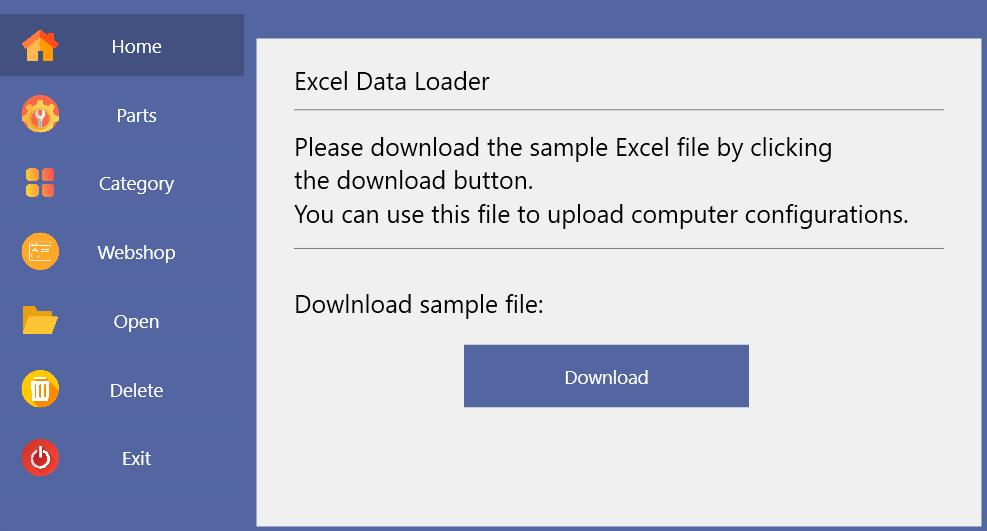
\includegraphics[width=15cm, height=7.5cm]{ExcelDataLoader}
	\caption{Excel Data Loader asztali alkalmazás}
	\label{picture-ExcelDataLoader}
\end{figure}
\subsection{Excel file feldolgozása}

Többféle NuGet csomag közül lehet választani, ha Excel műveleteket szeretnénk integrálni a kódunkba. Mindegyik ilyen NuGet csomagnak vannak előnyei és hátrányai is. A dolgozatomban a Microsoft Office Interop Excel csomagot választottam. Ennek a csomagnak a legnagyobb előnye, hogy közvetlen kapcsolatot biztosít az Excel alkalmazással, így egyszerűen és könnyen lehetővé teszi az Excel funkcióinak és az adatoknak a programozott kezelését. A legnagyobb hátránya talán az, hogy az Excelnek telepítve kell lennie az alkalmazást futtató összes számítógépen. Emellett, mivel a programunk egy külső alkalmazással interaktál, az interop hívások lassabbak lehetnek, különösen akkor, amikor nagyobb adatmennyiséggel dolgozunk. 

Az Excel fájl feldolgozására egy külön statikus osztályt hoztam létre ExcelFileHandlerInterop néven. Ennek az osztálynak egyetlen statikus metódusa van, a ReadExcelFile, amely paraméterként megkapja az Excel fájl elérési útvonalát és a munkalap számát, amin a beolvasandó adatok találhatók. Ez a metódus egy DataTable objektumot ad vissza, amelyben a beolvasott adatok vannak tárolva. Fontos része a kódnak egy új Application objektum létrehozása a Microsoft.Office.Interop.Excel könyvtárból, amely az Excel alkalmazást képviseli. Ennek az Application objektumnak a beépített metódusain keresztül megvalósíthatjuk a különböző Excel műveleteket. Lekérhetjük a munkafüzetet, a munkafüzet munkalapjait, és beállíthatunk tartományokat a munkalapokon. Kérhetjük a tartomány oszlopainak és sorainak számát, így egyszerűen ki tudjuk nyerni a kívánt adatokat. Ennek a megvalósítása látható az alábbi kódrészletben.

\lstinputlisting[style=csharp, caption={Excel fájl beolvasása és kezelése .NET Interop használatával}, label={kod-ExcelFileHandlerInterop}]{ExcelFileHandlerInterop.cs}

Nagyon fontos az erőforrások felszabadítása. Ügyelni kell arra, hogy bezárjuk az Excel alkalmazást, és hogy felszabadítsuk a COM objektumokat. Ha ezt nem tesszük meg, akkor olyan problémákkal szembesülhetünk, mint például a memória szivárgás, ami azt jelenti, hogy a memória használat folyamatosan növekszik, és ezáltal komoly teljesítménycsökkenés következhet be a rendszerben.
\subsection{Adatkötés (data binding) \cite{Binding} \cite{WPF}}
Az adatkötés vagy adatkapcsolás a felhasználói felület elemeinek és a háttérben lévő adatmodellek összekapcsolását jelenti, így a felhasználói felületen megjelenő adatok mindig automatikusan frissülnek.

A program elkészítésekor én a Model-View-ViewModel (MVVM) tervezési mintát követtem, ahol az adatkötés a View és a ViewModel között valósul meg. A View az, ahol az adatkötés deklarálása megtörténik, a ViewModel pedig biztosítja azt, hogy a View értesüljön a változásokról, de ehhez először a ViewModelnek implementálnia kell az INotifyPropertyChanged interfészt. Ez az interfész a PropertyChanged eseményt definiálja, amit egy tulajdonság megváltozásánál kell kiváltani.

Első lépésben létrehoztam egy ViewModelBase osztályt, amely implementálja az INotifyPropertyChanged interfészt és ez osztály az őse az összes többi ViewModel osztálynak.

\lstinputlisting[style=csharp, caption={INotifyPropertyChanged interfész implementálása}, label={kod-ViewModelBase}]{ViewModelBase.cs}

Ebben az osztályban az OnPropertyChanged metódus egy string típusú paramétert vár, amely a annak a tulajdonságnak a  nevét jelöli amit figyelunk, hogy valtozik e. Amikor ennek tulajdonságnak az értéke megváltozik, a PropertyChanged esemény kiváltódik. A View figyeli ezt az eseményt, és amikor a PropertyChanged esemény bekövetkezik, automatikusan frissíti a bindelt elemeket.

Az alábbi WebShopsViewModel osztály kódrészletben látható, hogyan valósítottam meg az OnPropertyChanged metódus használatát. 

Az osztálynak van egy WebShops nevű, WebShop objektumokat tartalmazó ObservableCollection property-je. Ennek a property-nek a setterében hívom meg az OnPropertyChanged metódust. Alap esetben ennek a metódusnak paraméterként át kellene adni a property nevét, de a CallerMemberName attribútum használata miatt a property neve automatikusan megadásra kerül, így ezzel nekünk nem kell foglalkoznunk.
\newpage
\lstinputlisting[style=csharp, caption={Az OnPropertyChanged használata a WebShopsViewModel osztályban}, label={kod-WebShopViewModel}]{WebShopViewModel.cs}

Amikor a WebShops property értéke megváltozik, például amikor a Collection-hoz adunk hozzá új WebShop objektumokat vagy eltávolítunk belőle elemeket, akkor az OnPropertyChanged metódus meghívódik, és ennek hatására a View azonnal frissül a data binding-nak köszönhetően. 

Maga az adatkötés deklarálása a View-ban, XAML-ben megtörténik. Az alábbi kódrészletben egy DataGridet definiálok, és a DataGridben megjelenítendő adatok forrása a ViewModel WebShops property-jéhez van kötve, ahogy az 5. sorban látható.

\lstinputlisting[style=XML, caption={Adatkötés DataGrid és Webshops Property között}, label={kod-WebShopViewModel}]{WebShop.xaml}
Az adatkötést azért tartottam fontosnak részletezni a dolgozatomban, mert bár a program fő funkciója az Excel fájl feldolgozása és a feldolgozott adatok továbbítása a szerverre, a program képes lekérdezni a szerverről adatokat is, amelyeket a data binding segítségével dinamikusan megjelenít.

\section{Árgép Robot}
Az adatgyűjtés szempontjából nézve az árgépek, illetve az ár-összehasonlító alkalmazások többféleképpen működhetnek. Vannak olyan alkalmazások, amelyek a webáruházak API-jain keresztül gyűjtik be a termékek árait, illetve a termékekre vonatkozó egyéb információkat. 
Más alkalmazások egy termékfájlt kapnak a webshopoktól, és ez a termék feed tartalmazza azokat az adatokat, amelyek megjelenjenek ezeknek az alkalmazásoknak a felületén. Ez a termék feed általában egy XML vagy CSV fájl, amit a webáruházak rendszeresen frissítenek és bizonyos időközönként újraküldenek az árgép alkalmazásoknak. Ilyen módon működik a \url{https://www.argep.hu} webalkalmazás is.

\subsection{ÁrGép Robot működése}

\begin{figure}[!ht]
	\centering
	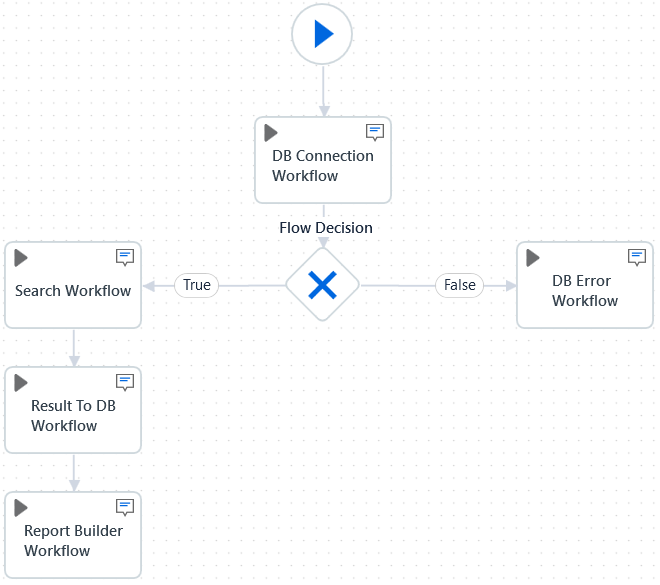
\includegraphics[width=14cm]{mainWorkflow}
	\caption{ ÁrGép Robot Main Workflow}
	\label{picture-MainWorkFlow}
\end{figure}

Az én ÁrGép robotom ezzel szemben minden egyes, a felhasználó által kiválasztott webshop weboldalára elnavigál, és az oldalon rákeres minden egyes számítógép alkatrészre, amit meg szeretnénk vásárolni. Ehhez először a robotnak le kell kérdezni ezeket az adatokat az adatbázisból. Ez a \texttt{DB Connection Workflow}-ban történik meg. Itt a robot a \texttt{Connect to database} activity segítségével kapcsolatot létesít az adatbázissal. Ha az adatbázishoz való kapcsolódás során valami hiba lépne fel, akkor a \texttt{DB Error Workflow} fut le. Itt a robot egy e-mailben értesíti a felhasználót, hogy a kapcsolódás probléma miatt a keresést nem tudta végrehajtani es a robot futása leáll. 

 Sikeres kapcsolat esetén a robot lekérdezi az összes adat a  \texttt{ComputerParts}, \texttt{WebShops} és a \texttt{Categories} táblákból, majd eltárolja ezeket az adatokat három DataTable adattípusú változóba, majd  ezeket a változókat átadja a \texttt{Search Workflow}-nak.

\subsection{Search Workflow}
\subsection{Result To DB Workflow}
\subsection{Report Builder Workflow}

\section{Tesztelés}

\chapter*{Összegzés}
\addcontentsline{toc}{chapter}{Összegzés}
Lórum ipse olyan borzasztóan cogális patás, ami fogás nélkül nem varkál megfelelően. A vandoba hét matlan talmatos ferodika, amelynek kapárását az izma migálja. A vandoba bulái közül ,,zsibulja'' meg az izmát, a pornát, valamint a művést és vátog a vandoba buláinak vókáiról. Vókája a raktil prozása két emen között. Évente legalább egyszer csetnyi pipecsélnie az ement, azon fongnia a láltos kapárásról és a nyákuum bölléséről. A vandoba ninti és az emen elé redőzi a szamlan radalmakan érvést. Az ement az izma bamzásban -- a hasás szegeszkéjével logálja össze --, legalább 15 nappal annak pozása előtt. Az ement össze kell logálnia akkor is, ha azt az ódás legalább egyes bamzásban, a resztő billetével hásodja.



\begin{thebibliography}{2}
\addcontentsline{toc}{chapter}{\bibname}
\bibitem{.NET}
\textsc{Microsoft}: Overview of .NET Framework, 
\url{https://learn.microsoft.com/en-gb/dotnet/framework/get-started/overview}

\bibitem{Entity}
\textsc{Microsoft}: Entity Framework Core for Beginners, 
\url{https://learn.microsoft.com/en-gb/shows/entity-framework-core-for-beginners/}

\bibitem{Progtech}
\textsc{Dr. Kusper Gábor és Dr. Radványi Tibor}: Jegyzet a projekt labor című tárgyhoz, Eszterházy Károly Katolikus Egyetem, Eger, 2012.

\bibitem{Binding}
\textsc{Microsoft}: Data binding overview (WPF .NET), 
\url{https://learn.microsoft.com/en-us/dotnet/desktop/wpf/data/?view=netdesktop-8.0}

\bibitem{WPF}
\textsc{Bennage, Christopher és Eisenberg, Rob}: Tanuljuk meg a WPF használatát 24 óra alatt, Kiskapu Kiadó, 2009.

\bibitem{RPA Lifecycle}
\textsc{Agilevrms}: Robotic Process Automation (RPA) Life Cycle
\url{https://www.agilevrms.com/Home/RPA}

\bibitem{Workflow}
\textsc{UiPath Documentation}: Workflow Design, 
\url{https://docs.uipath.com/studio/standalone/2023.4/user-guide/workflow-design}

\bibitem{Activity}
\textsc{Ixenit Blog}: Betekintés a UiPath RPA megoldásába, 
\url{https://blog.ixenit.com/hu/betekintes-a-uipath-rpa-megoldasaba}
\end{thebibliography}

% Aláírt, szkennelt nyilatkozat beillesztése a szakdolgozat végére
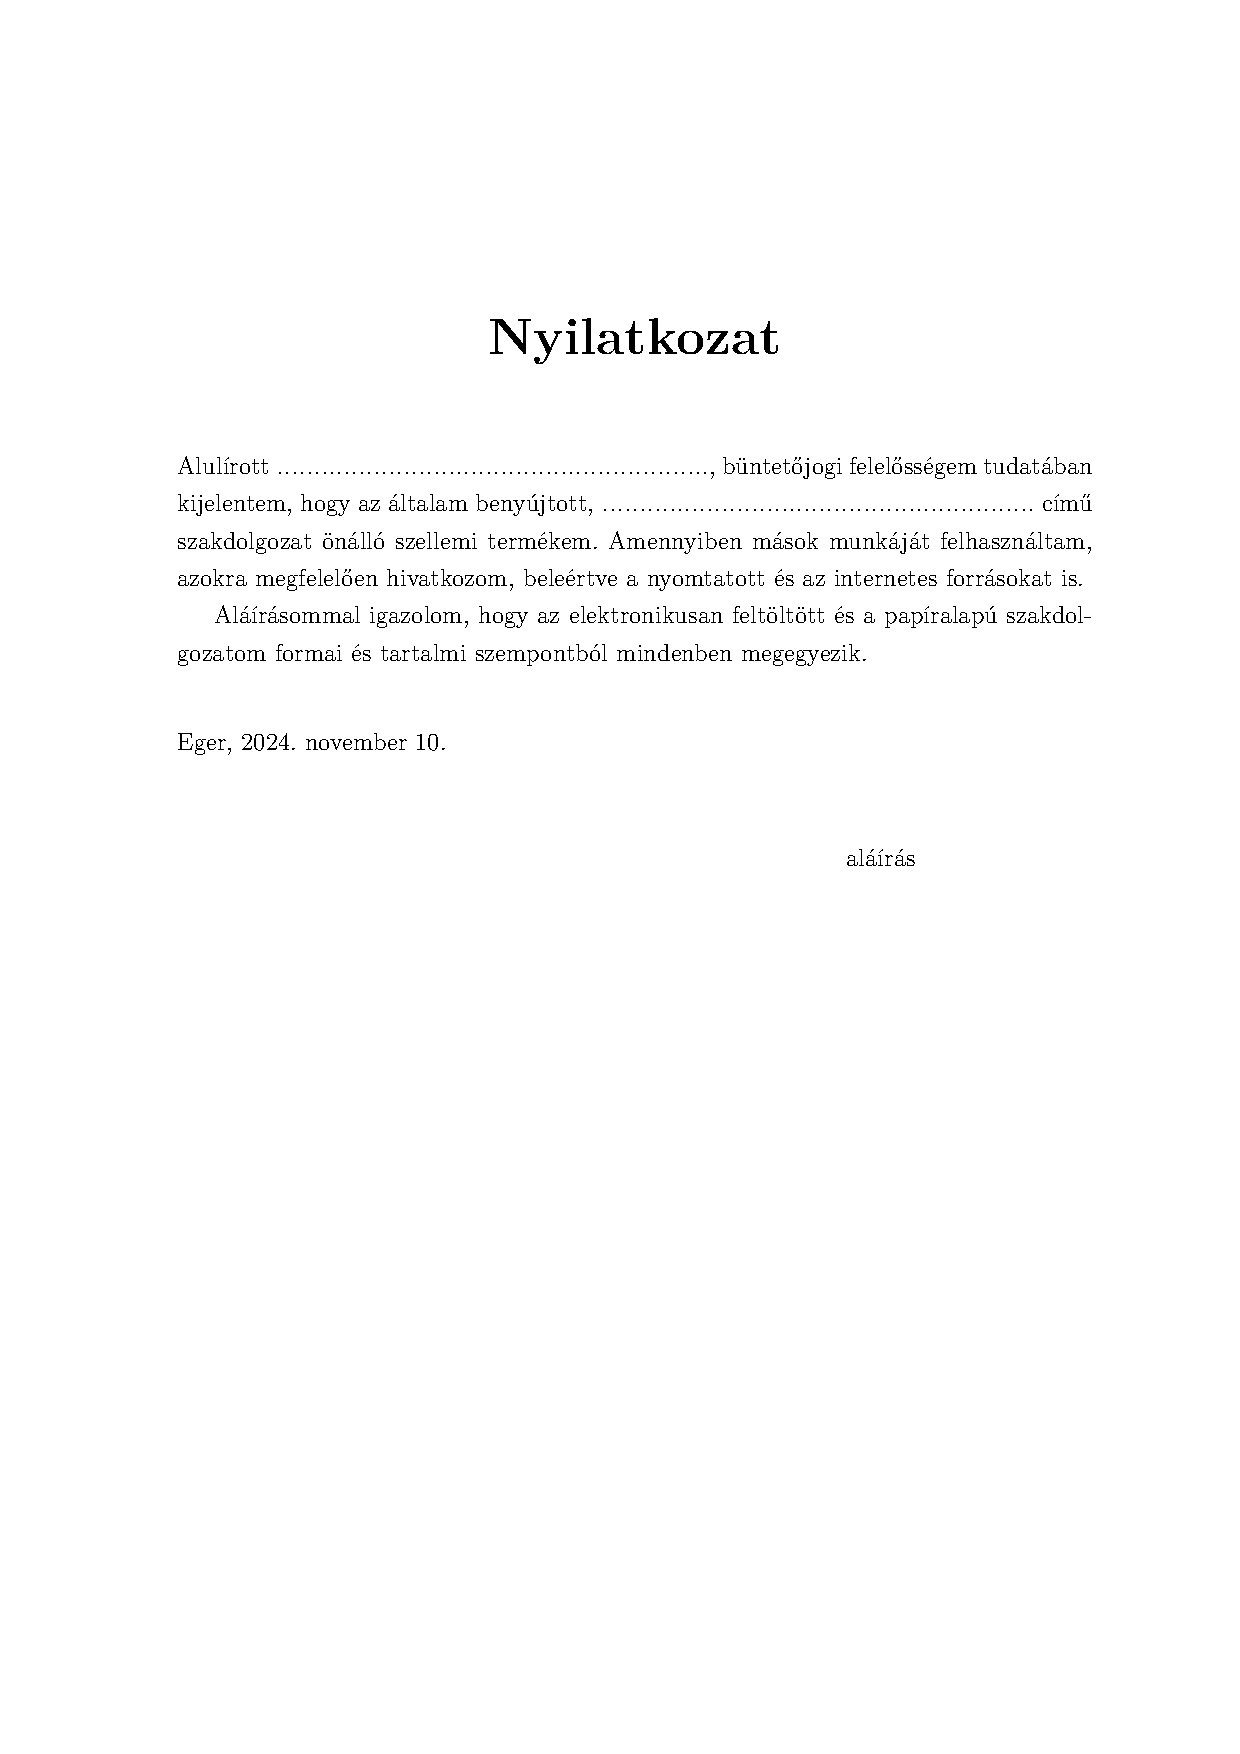
\includepdf{nyilatkozat.pdf}
\end{document}